\documentclass{article}

\usepackage{graphicx}
\usepackage[utf8]{inputenc}
\usepackage[T1]{fontenc}
\usepackage[french]{babel}
\usepackage{hyperref}
\usepackage{amsmath,amsfonts,amssymb}
%\usepackage{Tkz-Tab}
\usepackage{wrapfig}
\usepackage{verbatim}
\usepackage{array}

\begin{document}

\title{Gestion de flux dans le réseau
	\smallbreak
	TD n\degre6
	\smallbreak
	Modélisation mathématique
	\smallbreak
	Q4}
\author{Sibylle Roux \and Juliette Arazo \and Nicolas Le Gallo \and Tanguy Thomas}

\maketitle

\newpage

\tableofcontents

\newpage

\section{Etude de la file M/M/1}


\subsection{Conception d'une représentation informatique}
\paragraph{}
Pour stocké les valeurs simulés on utilisera un tableau de la forme : 
\begin{center}
\begin{tabular}{lll}
\hline
\hline
instant $t$ & $q(t)$ & incrément \\
\hline
\hline
\end{tabular}
\end{center}
\paragraph{}
Cette représentation est idéale : elle réunit toutes les informations utiles du fonctionnement des serveurs : 
\begin{itemize}
	\item l'instant où se passe l'evenement
	\item le type d'evenement (entrée ou sortie d'un client dans le système)
	\item le nombres de clients présent dans le système
\end{itemize}
Cette dernière valeur nous sera utile pour avoir la taille de la fille d'attente : 
\begin{align}
	taille\_file=max(q(t)-1,0)
\end{align}

\subsection{Conception et développement d'un algorithme de simulation en scilab}
Nous avons à notre disposition une fonction SciLab $insere(q, ta, ts)$ avec :
\begin{itemize}
	\item \textbf{q} : Matrice de notre représentation informatique de la file
	\item \textbf{ta} : Temps actuel
	\item \textbf{ts} : Temps de service
\end{itemize}
\begin{verbatim}
function newq = insere(q, ta, ts)
    if q($, 1) < ta then // aucune requête dans le système
        q($+1,:) = [ta, 1, 1]; // ajout de la requête en fin de liste
    else // inscription de la requête en file d'attente
        ind = sum(q(:, 1) < ta); // recherche du point d'insertion
        q(ind+2:$+1, :) = q(ind+1:$, :); // création d'un trou pour insérer
        q(ind+1,:) = [ta, q(ind,2), 1]; // insertion au bon endroit
        q(ind+1:$,2) = q(ind+1:$,2) + 1; // correction de la taille de
                                         // la file pour les lignes suivantes
    end
    // Inscription du départ de la requête après son temps de
    // service ts
    s = q($, 1) + ts // calcul de la date de sortie
    q($+1, :) = [s, q($, 2) - 1, -1]; // inscription de la date de sortie à la fin
    newq = q // On renvoie la file ainsi modifiée
endfunction
\end{verbatim}
\paragraph{}
Nous avons aussi la fonction $randExp(n,lambda)$ qui genere un vecteur de taille $n$ de valeurs aléatoires suivant la loi exponentielle de paramètre $\lambda=lambda$
\begin{verbatim}
function t = randExp(n, lambda)
    t = -log(1 - rand(n,1)) / lambda
endfunction
\end{verbatim}

\paragraph{}
C'est à l'aide de ces deux fonctions citées plus haut que l'on peut définir la fonction : $queue(Tmax, lambda, mu)$ où :
\begin{itemize}
	\item \textbf{Tmax} : Instant maximal de la représentation de la file
	\item \textbf{lambda} : $\lambda$ correspondant aux temps inter-arrivées
	\item \textbf{mu} :  $\lambda$ correspondant aux temps de service
\end{itemize}
\begin{verbatim}
function a=queue(Tmax, lambda, mu)
    Q = [0, 0, 0]; // Initialisation de la file
    t = 0; // temps courant
    while (t < Tmax)
        t_ia=randExp(1,lambda); // tirage de l'intervalle inter-arrivée
        t=t+t_ia;// mise à jour de l'instannt courant : 
                 // instant d'arrivée de la prochaine requête
        ts=randExp(1,mu); // tirage de son temps de service
        Q=insere(Q,t,ts);// insertion dans la file des évènements
    end
    a = Q (Q(:,1)<Tmax,:) // on renvoie l'état de la file à la date Tmax
endfunction
\end{verbatim}

\subsection{Simulation de trajectoires}

\subsubsection{Simulation de l'évolution d'un file d'attente}
\paragraph{}
Pour simuler les différentes trajectoires, on va utiliser une fonction Scilab $traj(n,lambda,mu)$ où :
\begin{itemize}
	\item \textbf{n} : correspondant à l'instant maximal de la représentation de la file
	\item \textbf{lambda} : $\lambda$ correspondant aux temps inter-arrivées
	\item \textbf{mu} :  $\lambda$ correspondant aux temps de service
\end{itemize}
\begin{verbatim}
function traj(n,lambda,mu)
    for i=1:50 // 50 trajectoires
        Q = queue(n, lambda, mu); // lambda est 5 fois plus grand que mu
        plot2d2(Q(:,1), max(Q(:,2) - 1, 0), style=2) // trace la courbe
    end
endfunction
\end{verbatim}

\subsubsection{Distribution statistiques de la taille de la file d'attente}
\paragraph{}
Pour avoir la distribution statistique de des trajectoires, on va utiliser une fonction Scilab $distrib(n,lambda,mu)$ où :
\begin{itemize}
	\item \textbf{n} : correspondant à l'instant maximal de la représentation de la file
	\item \textbf{lambda} : $\lambda$ correspondant aux temps inter-arrivées
	\item \textbf{mu} :  $\lambda$ correspondant aux temps de service
\end{itemize}
\begin{verbatim}
function Qi=distrib(n,lambda,mu)
    Qi = zeros(500, 1);
    for i=1:500
        Q = queue(n, lambda, mu);
        Qi(i) = Q($, 2);
    end
    distr = tabul(Qi,'i')
    bar(distr(:,1),distr(:,2)/500)
    legend("Distribution de Q"+string(n))
endfunction
\end{verbatim}
\paragraph{}
Lorsque l'amplitude sera très grande, on optera plutôt pour une autre version de cette fonction $distribv2(n,lambda,mu)$: 
\begin{verbatim}
function Qi=distribv2(n,lambda,mu)
    Qi = zeros(500, 1);
    for i=1:500
        Q = queue(n, lambda, mu);
        Qi(i) = Q($, 2);
    end
    histplot(20,Qi)
    legend("Distribution de Q"+string(n))
endfunction
\end{verbatim}

\subsubsection{Temps de service supérieur en moyenne aux temps inter-arrivées}
\paragraph{Paramètre : $n=60$ ; $lambda=0.5$ ; $mu=0.2$}
\begin{center}
	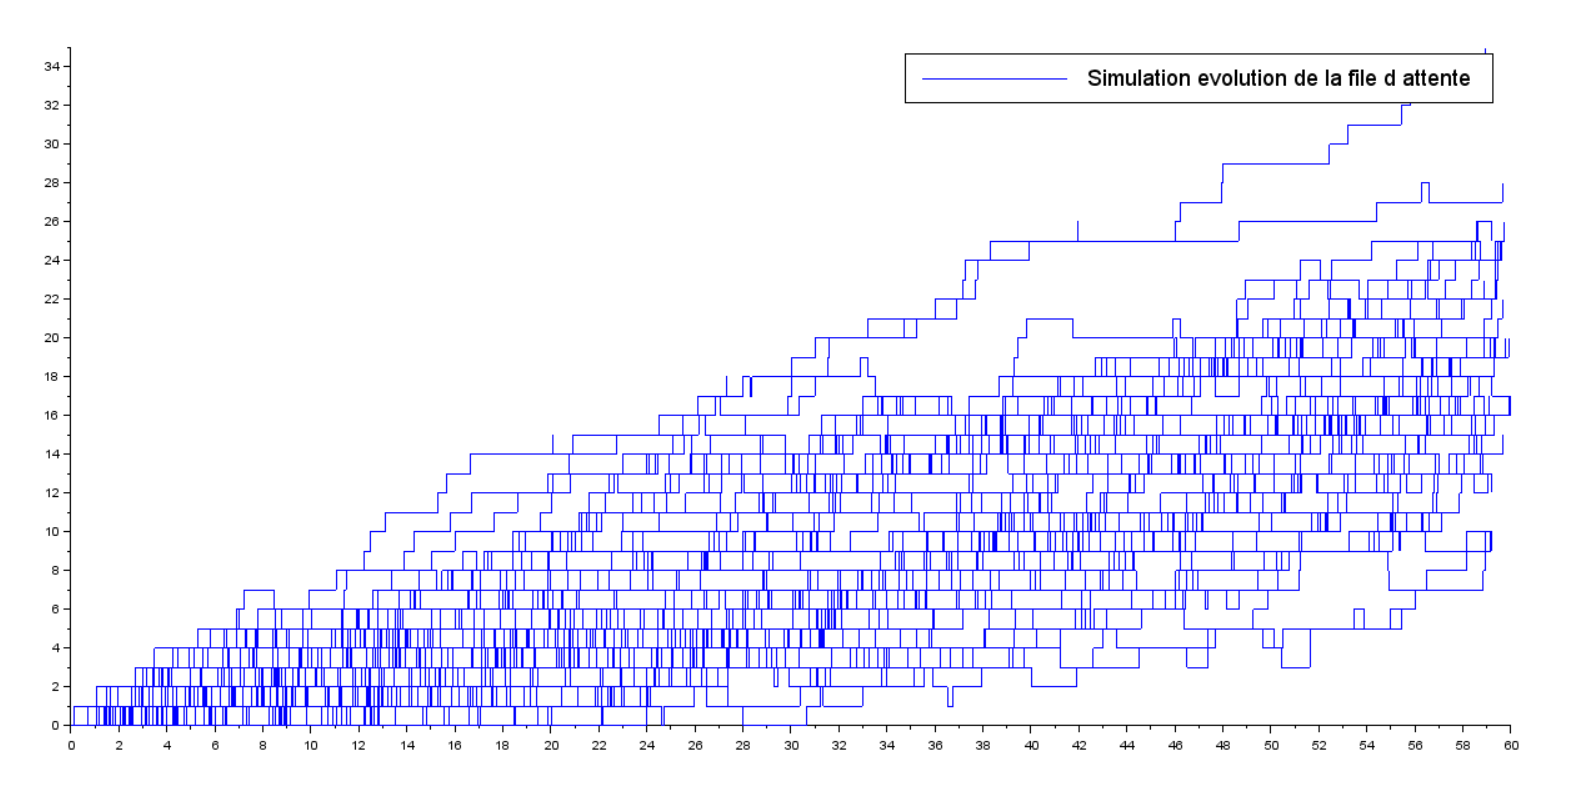
\includegraphics[width=425px]{img/inf.PNG}
\end{center}
\begin{center}
	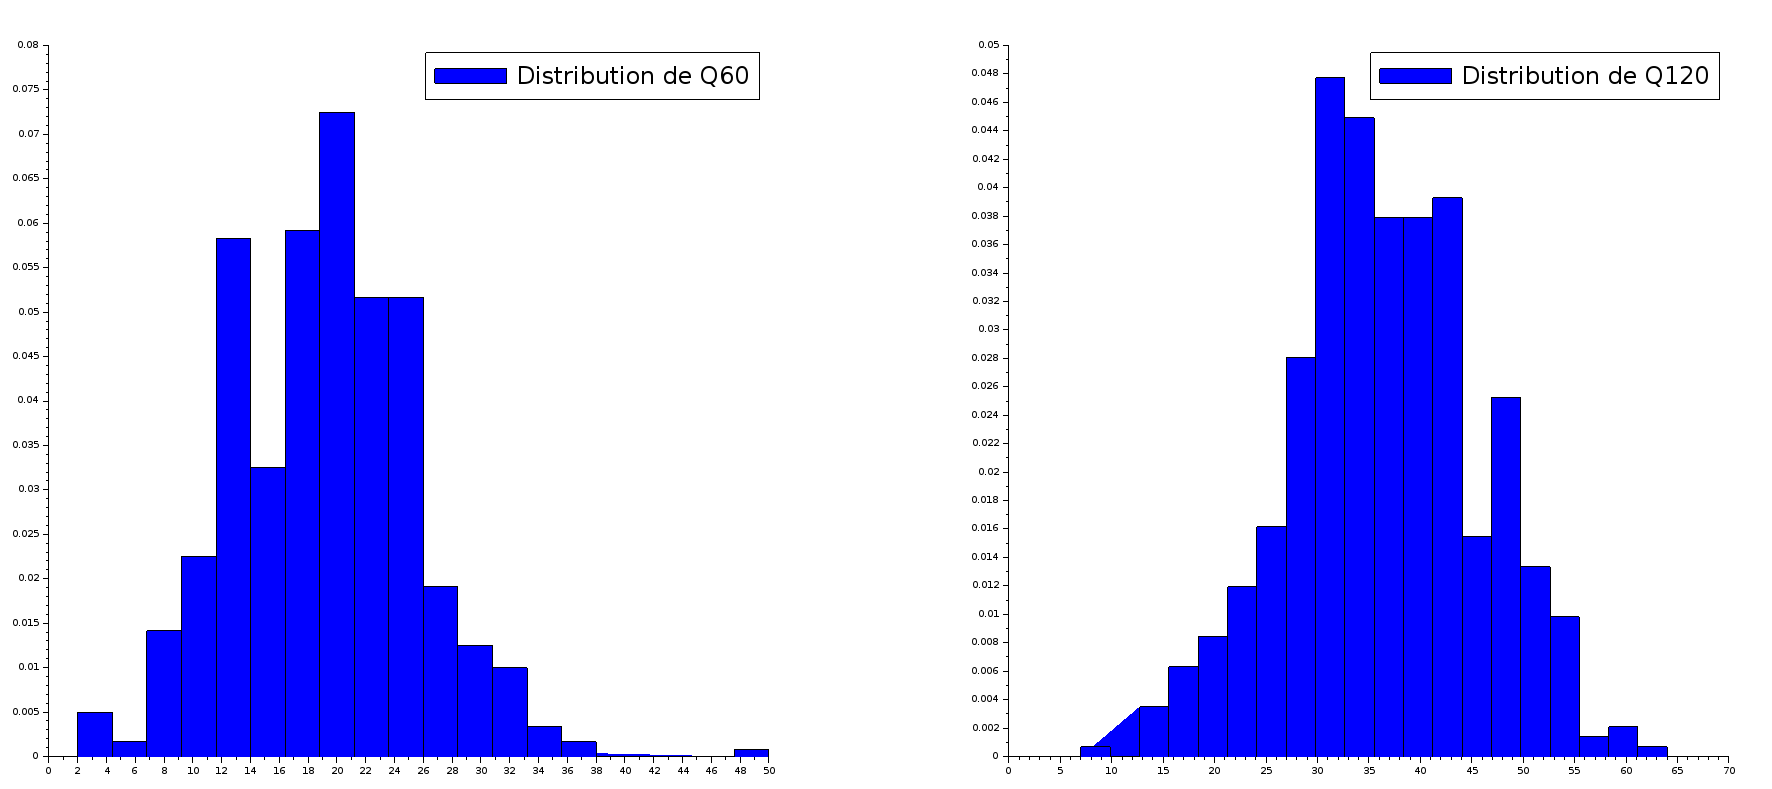
\includegraphics[width=425px]{img/sup/dist.png}
\end{center}
\begin{center}
	\begin{tabular}{c||c||c}
		& Q60 & Q120 \\
		\hline \hline
		mean() & 18.54 & 36.806 \\
		\hline \hline
		variance() & 40.212826 & 81.158681 \\
	\end{tabular}
\end{center}

\subsubsection{Temps de service inférieur en moyenne aux temps inter-arrivées}
\paragraph{Paramètre : $n=60$ ; $lambda=0.2$ ; $mu=0.5$}
\begin{center}
	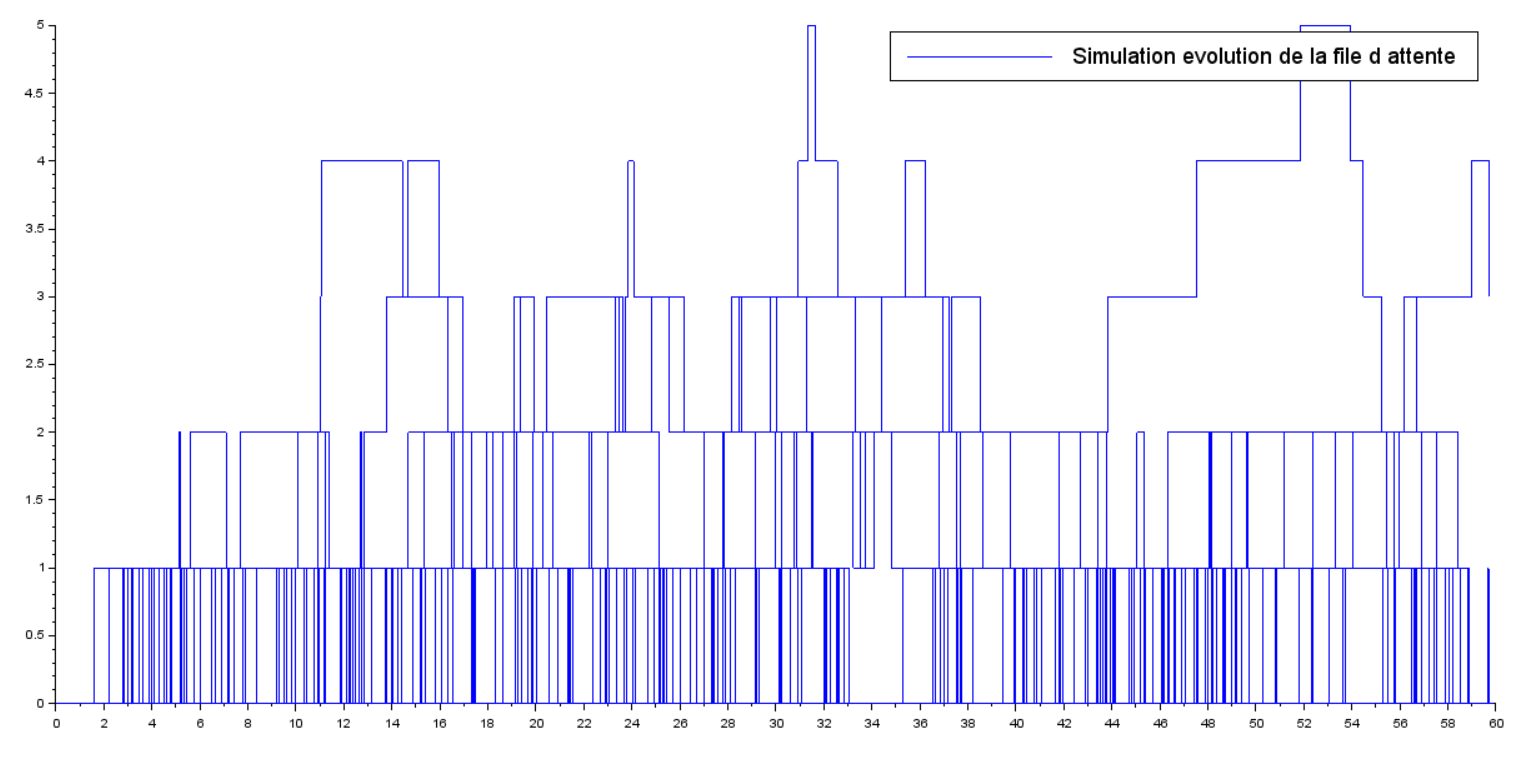
\includegraphics[width=425px]{img/sup.PNG}
\end{center}
\begin{center}
	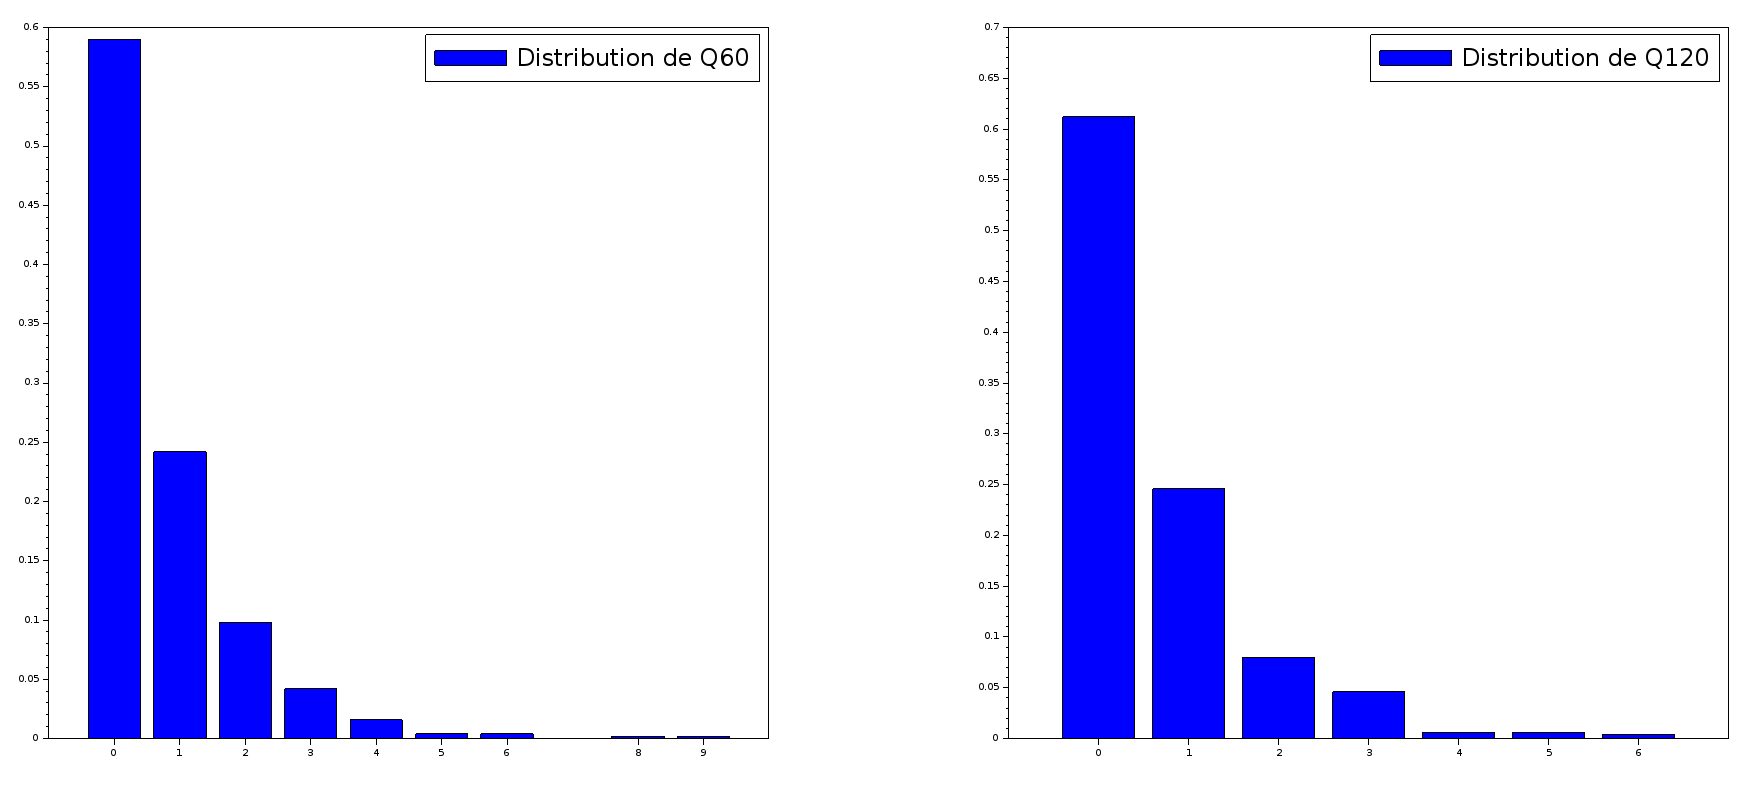
\includegraphics[width=425px]{img/inf/dist.png}
\end{center}
\begin{center}
	\begin{tabular}{c||c||c}
		& Q60 & Q120 \\
		\hline \hline
		mean() & 0.582 & 0.704 \\
		\hline \hline
		variance() & 0.9611984 & 1.1787415 \\
	\end{tabular}
\end{center}

\subsubsection{Temps de service égaux en moyenne aux temps inter-arrivées}
\paragraph{Paramètre : $n=60$ ; $lambda=0.5$ ; $mu=0.5$}
\begin{center}
	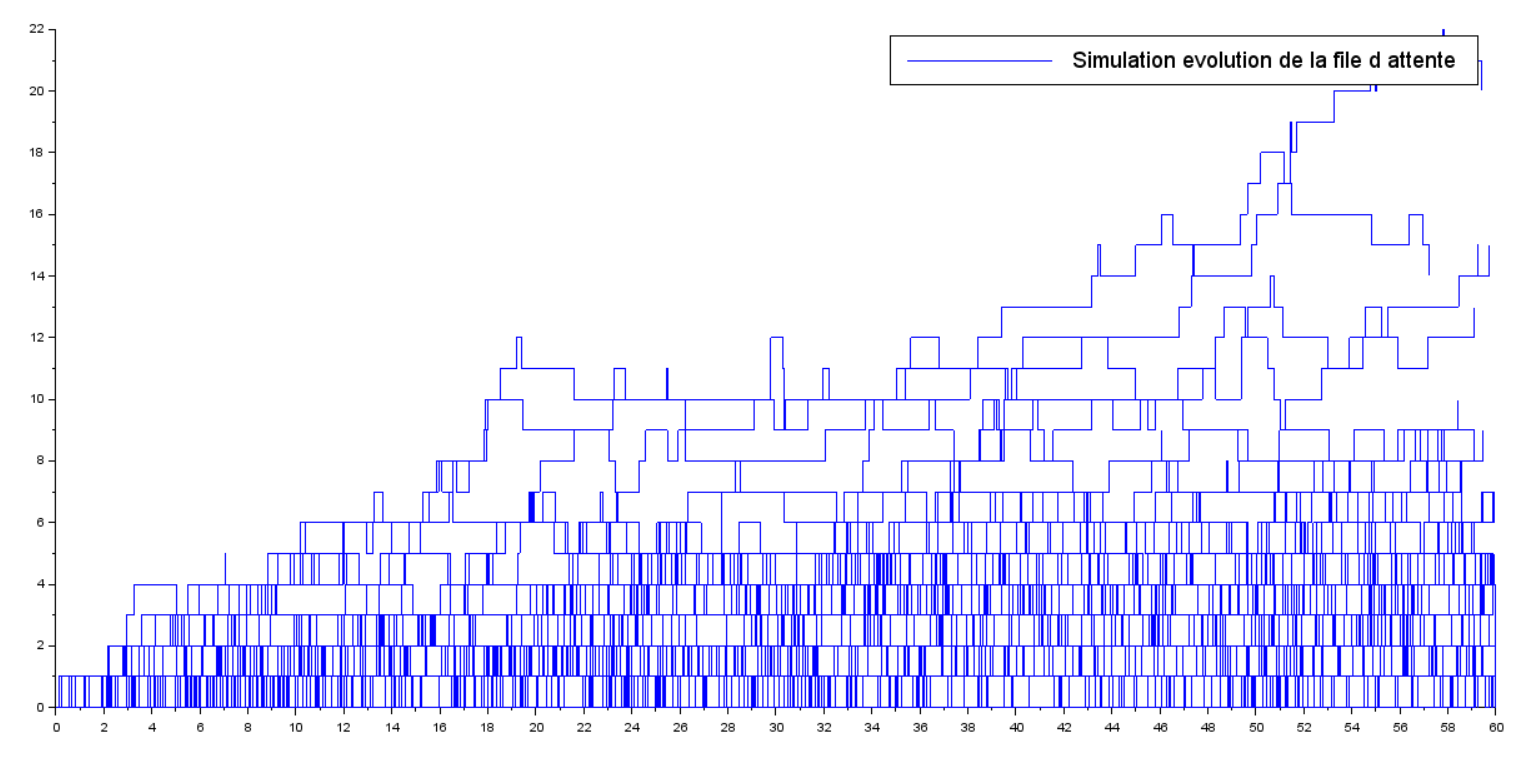
\includegraphics[width=425px]{img/egal.PNG}
\end{center}
\begin{center}
	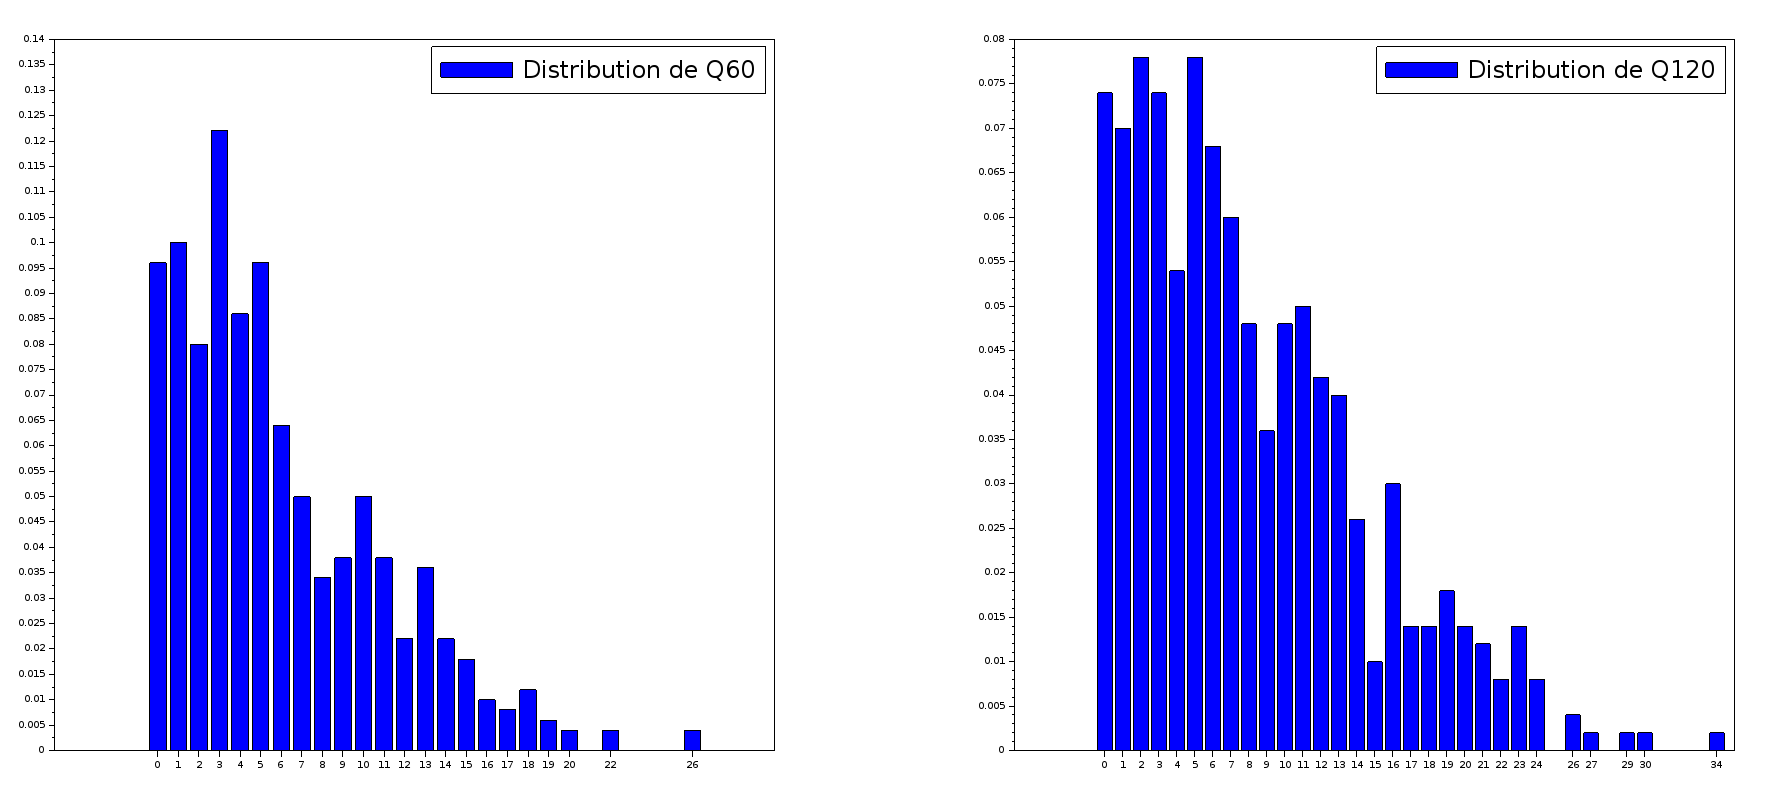
\includegraphics[width=425px]{img/egal/dist.png}
\end{center}
\begin{center}
	\begin{tabular}{c||c||c}
		& Q60 & Q120 \\
		\hline \hline
		mean() & 5.726 & 8.476 \\
		\hline \hline
		variance() & 24.792509 & 46.350124 \\
	\end{tabular}
\end{center}


\section{Etude de la file à 3 serveurs}

\subsection{Simulation de stratégie circulaire}
\paragraph{}
Pour simuler la stratégie circulaire, on va utiliser la fonction $circul(Tmax,lambda,mu)$ où :
\begin{itemize}
	\item \textbf{Tmax} : Durée en seconde de la simulation
	\item \textbf{lambda} : $\lambda$ correspondant aux temps inter-arrivées
	\item \textbf{mu} : vecteur contenant les $\lambda$ correspondant aux temps de service des 3 serveurs
\end{itemize}
\begin{verbatim}
function [Q1, Q2, Q3] = circul(Tmax, lambda, mu)
    Q1 = [0, 0, 0]; Q2 = Q1; Q3 = Q1;
    i = 0; 
    ta = 0; 
    while (ta < Tmax)
        ia = randExp(1, lambda) 
        i = i+1 
        ta = ta + ia
        nq = modulo(i, 3) + 1
        ts = randExp(1, mu(nq))
        select nq 
        case 1.
            Q1 = insere(Q1, ta, ts)
        case 2 
            Q2 = insere(Q2, ta, ts)
        else
            Q3 = insere(Q3, ta, ts)
        end
    end
    Q1 = Q1(Q1(:,1)<Tmax,:)
    Q2 = Q2(Q2(:,1)<Tmax,:) 
    Q3 = Q3(Q3(:,1)<Tmax,:) 
endfunction 
\end{verbatim}

\paragraph{}
Dans cette fonction, on utilise 2 autres fonctions : 

\begin{itemize}
	\item $insere(q, ta, ts)$ où :
	\begin{itemize}
		\item \textbf{q} : File d'attente
		\item \textbf{ta} : Instant d'arrivée de la requête
		\item \textbf{ts} : Temps de service
	\end{itemize}
	\item $randExp(n, lambda) $
	\begin{itemize}
		\item \textbf{n} : taille du vecteur en sortie
		\item \textbf{lambda} : $\lambda$ avec lequel sera générée la valeur aléatoire qui suit une loi exponentielle
	\end{itemize}
\end{itemize}

\begin{center}
	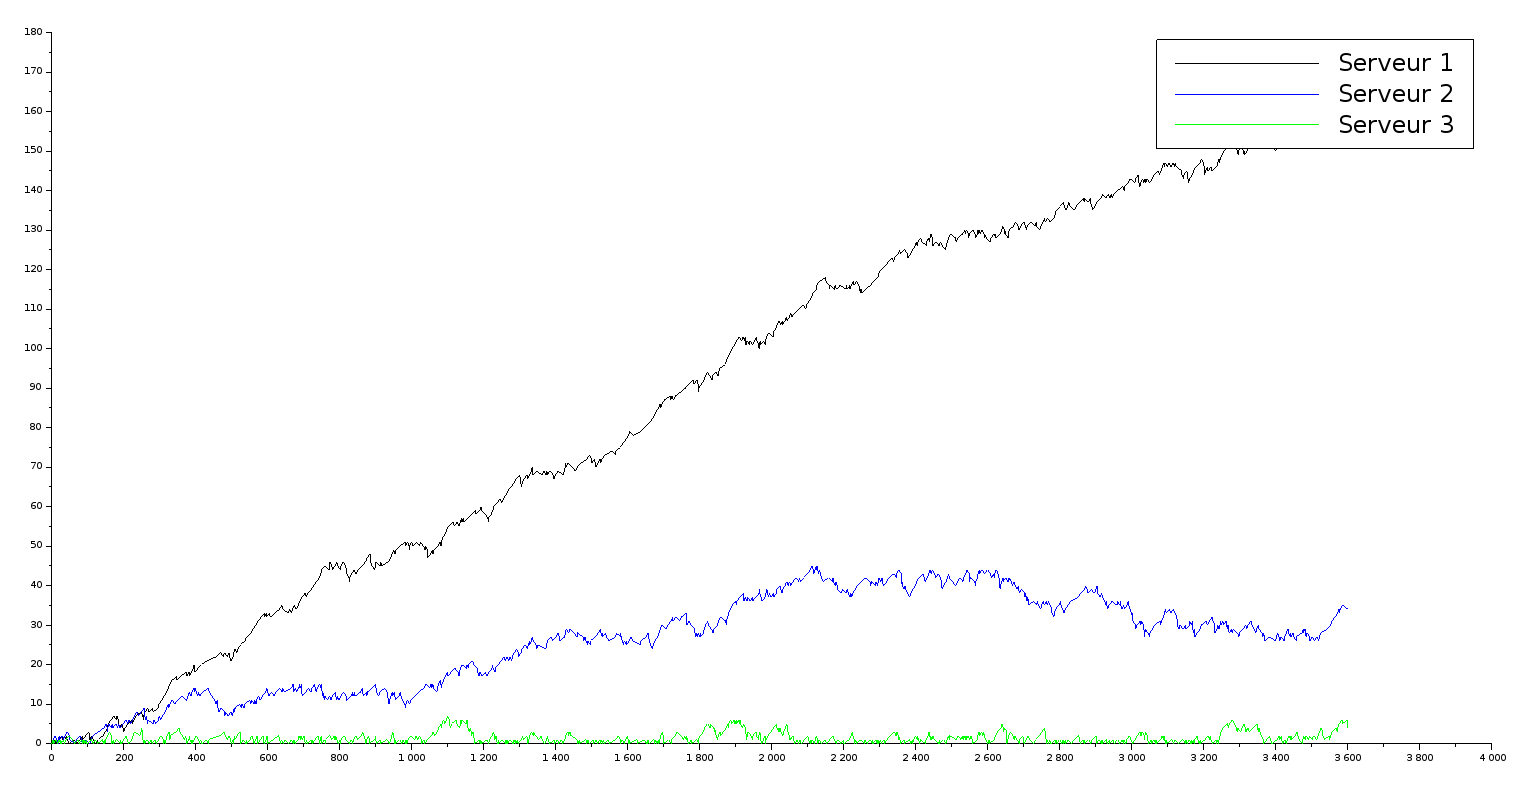
\includegraphics[width=425px]{img/circul1h.png}
\end{center}
\paragraph{Simulation sur 1 heure}

\begin{center}
	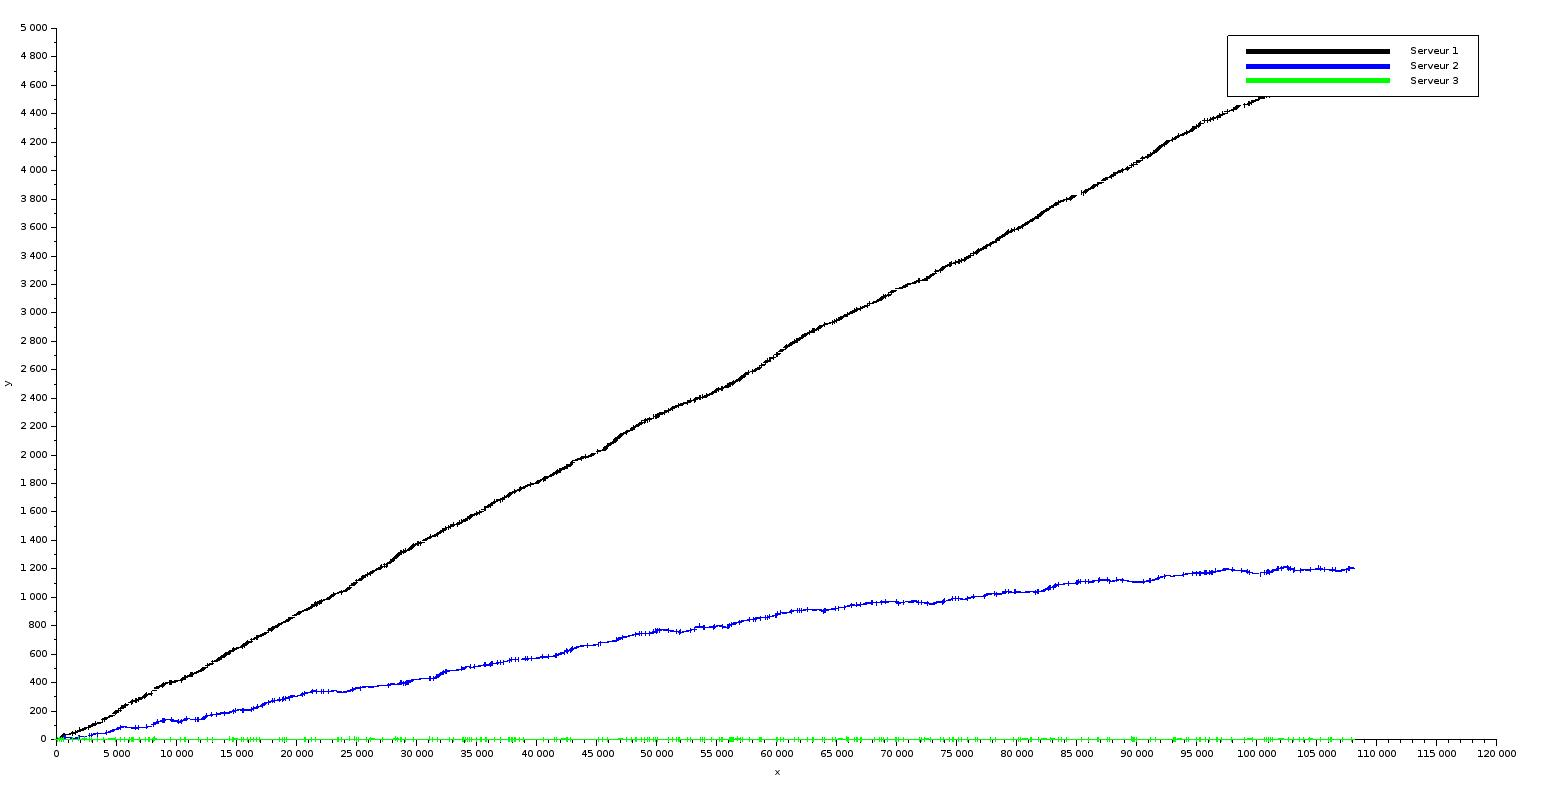
\includegraphics[width=425px]{img/circul30h.jpg}
\end{center}
\paragraph{Simulation sur 30 heures}

\subsubsection{Etude numérique du temps de traversée du système pour une requête}
\subsubsection{Etude numérique du nombre de requêtes dans le système}
\subsubsection{Recherche d'un régime stationnaire}

\subsection{Simulation de la stratégie d'affection aléatoire proportionnelle}
\subsubsection{Simulation}
\subsubsection{Etude numérique}

\subsection{Autres stratégies, aléatoires ou/et détérministes}

\section{Conclusion}
\paragraph{}

\newpage
\appendix

\section{Fonctions}

\subsection{insere(q,ta,ts)}
\begin{verbatim}
function newq = insere(q, ta, ts)
    if q($, 1) < ta then 
        q($+1,:) = [ta, 1, 1];
    else
        ind = sum(q(:, 1) < ta);
        q(ind+2:$+1, :) = q(ind+1:$, :);
        q(ind+1,:) = [ta, q(ind,2), 1];
        q(ind+1:$,2) = q(ind+1:$,2) + 1;
    end
    s = q($, 1) + ts 
    q($+1, :) = [s, q($, 2) - 1, -1];
    newq = q
endfunction
\end{verbatim}

\subsection{randExp(n,lambda)}
\begin{verbatim}
function t = randExp(n, lambda)
    t = -log(1 - rand(n,1)) / lambda
endfunction
\end{verbatim}

\subsection{}
\begin{verbatim}
\end{verbatim}

\end{document}